% SkyHand pipeline: glove data -> training -> 30 Hz inference -> drone.
% Build: tectonic docs/pipeline.tex && pdftocairo -svg docs/pipeline.pdf docs/pipeline.svg
\documentclass[border=8pt]{standalone}
\usepackage[T1]{fontenc}
\usepackage{helvet}
\renewcommand{\familydefault}{\sfdefault}
\usepackage{tikz}
\usetikzlibrary{positioning, arrows.meta, fit, backgrounds, calc}

\definecolor{sense}{HTML}{3B82C4}
\definecolor{train}{HTML}{8E6CC9}
\definecolor{run}{HTML}{2E9E6A}
\definecolor{pre}{HTML}{3A9DA6}
\definecolor{llm}{HTML}{D9822B}
\definecolor{safe}{HTML}{C8433B}
\definecolor{ink}{HTML}{222222}

\tikzset{
  box/.style={draw=#1, fill=#1!10, rounded corners=3pt, line width=0.8pt, align=center,
              text width=3.15cm, minimum height=1.45cm, font=\small, text=ink},
  note/.style={font=\scriptsize, text=ink!75, align=center},
  flow/.style={-{Stealth[length=5pt]}, line width=0.9pt, draw=ink!70},
  off/.style={flow, dashed},
  lane/.style={draw=#1!60, fill=#1!3, rounded corners=6pt, line width=0.6pt, inner sep=9pt},
  lanetitle/.style={font=\bfseries\small, text=#1, anchor=south west},
}

\begin{document}
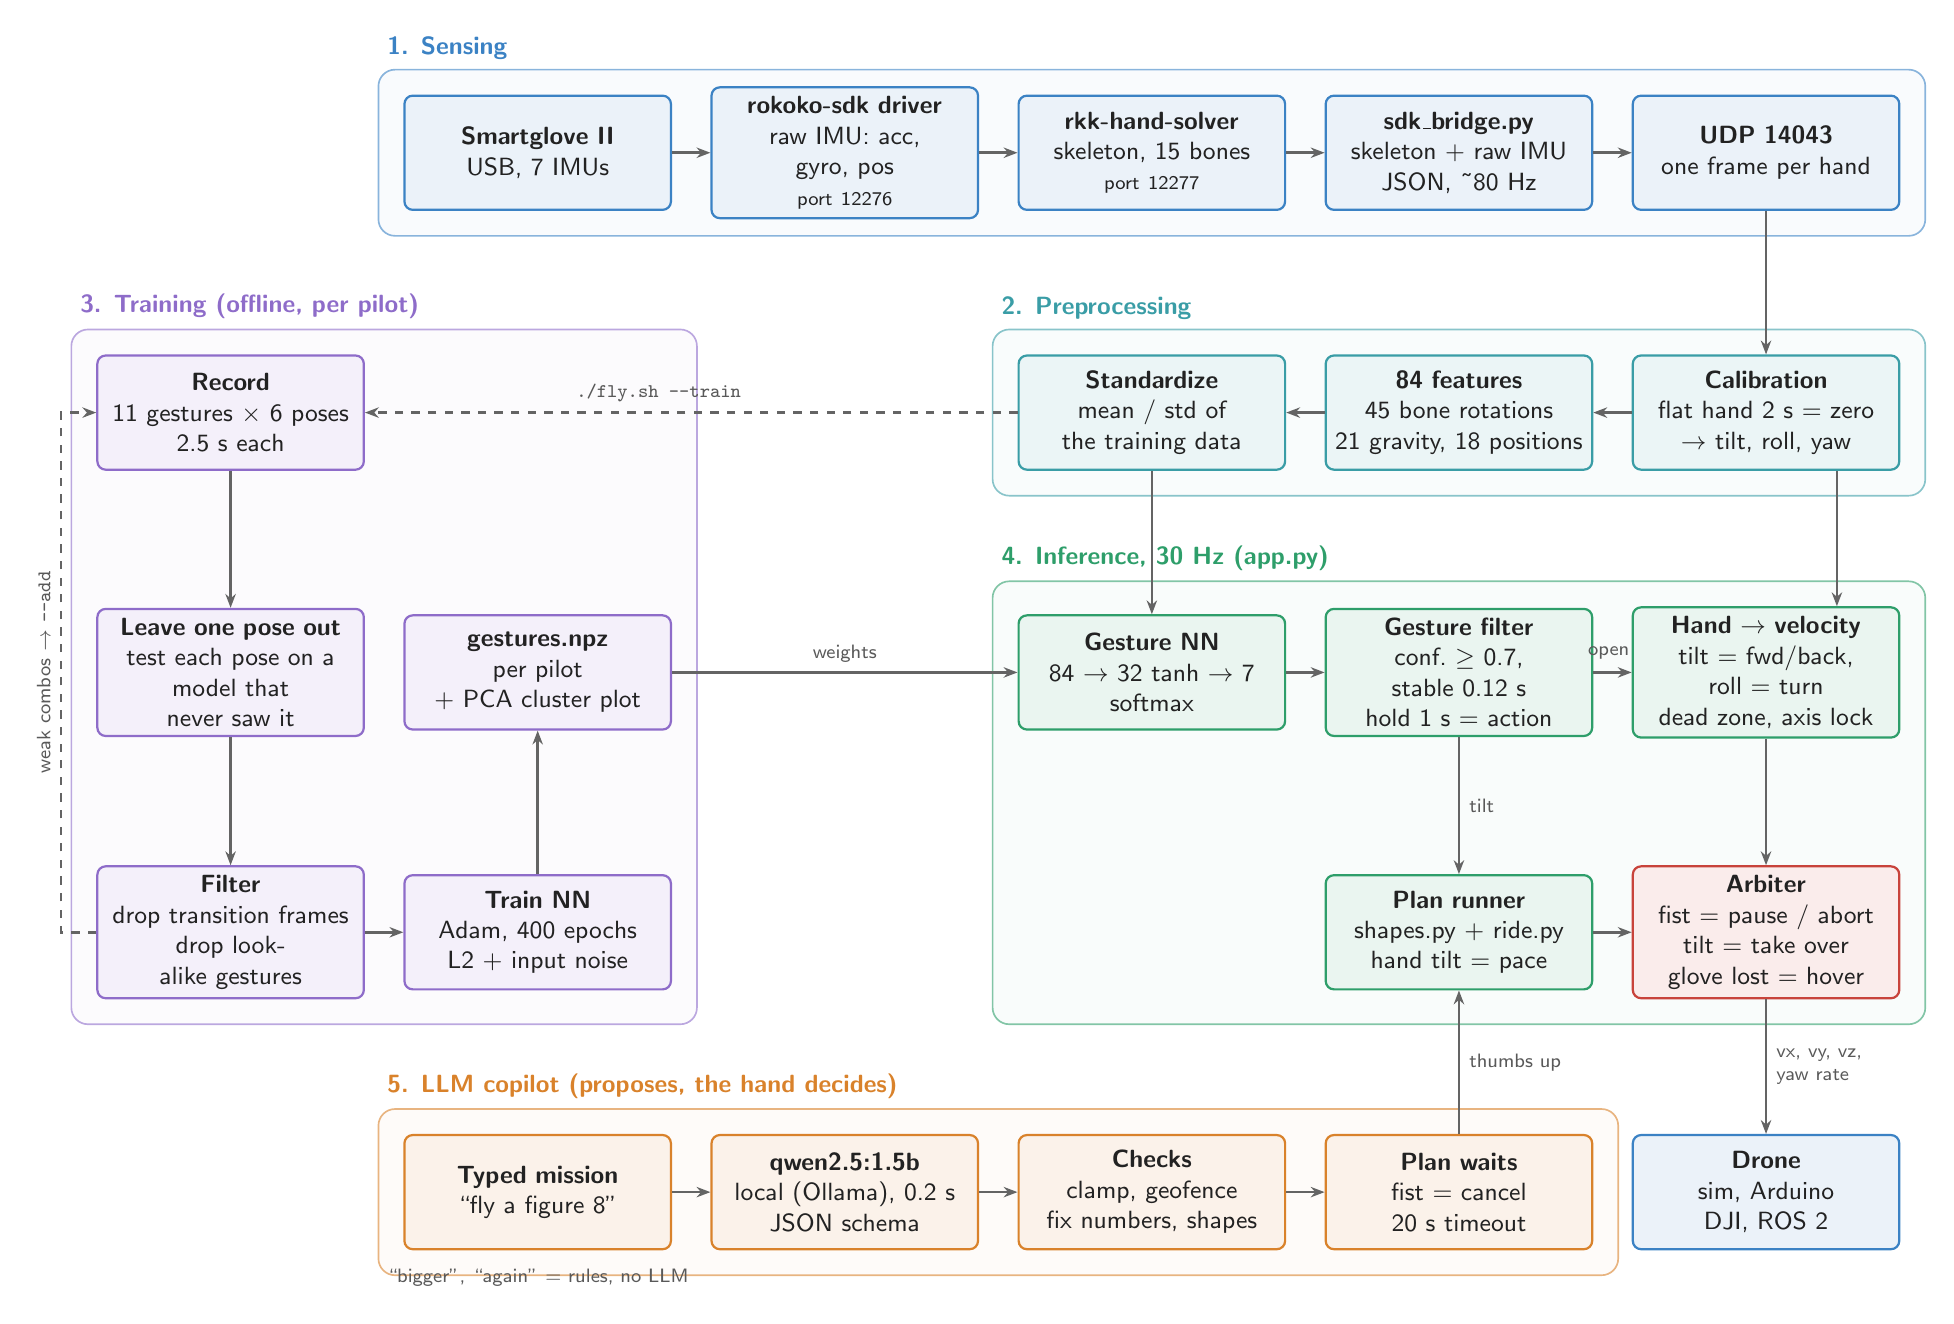
\begin{tikzpicture}
\def\cx#1{#1*3.9}  % column spacing
\def\ry#1{-#1*3.3}  % row spacing

% ---------- 1. sensing ----------
\node[box=sense] (glove)  at (\cx{1},\ry{0}) {\textbf{Smartglove II}\\ USB, 7 IMUs};
\node[box=sense] (driver) at (\cx{2},\ry{0}) {\textbf{rokoko-sdk driver}\\ raw IMU: acc, gyro, pos\\ \scriptsize port 12276};
\node[box=sense] (solver) at (\cx{3},\ry{0}) {\textbf{rkk-hand-solver}\\ skeleton, 15 bones\\ \scriptsize port 12277};
\node[box=sense] (bridge) at (\cx{4},\ry{0}) {\textbf{sdk\_bridge.py}\\ skeleton + raw IMU\\ JSON, \textasciitilde80 Hz};
\node[box=sense] (udp)    at (\cx{5},\ry{0}) {\textbf{UDP 14043}\\ one frame per hand};
\draw[flow] (glove) -- (driver);
\draw[flow] (driver) -- (solver);
\draw[flow] (solver) -- (bridge);
\draw[flow] (bridge) -- (udp);

% ---------- 2. preprocessing ----------
\node[box=pre] (calib) at (\cx{5},\ry{1}) {\textbf{Calibration}\\ flat hand 2 s = zero\\ $\to$ tilt, roll, yaw};
\node[box=pre] (feat)  at (\cx{4},\ry{1}) {\textbf{84 features}\\ 45 bone rotations\\ 21 gravity, 18 positions};
\node[box=pre] (std)   at (\cx{3},\ry{1}) {\textbf{Standardize}\\ mean / std of\\ the training data};
\draw[flow] (udp) -- (calib);
\draw[flow] (calib) -- (feat);
\draw[flow] (feat) -- (std);

% ---------- 3. training (offline) ----------
\node[box=train] (rec)   at (\cx{0},\ry{1}) {\textbf{Record}\\ 11 gestures $\times$ 6 poses\\ 2.5 s each};
\node[box=train] (loo)   at (\cx{0},\ry{2}) {\textbf{Leave one pose out}\\ test each pose on a\\ model that never saw it};
\node[box=train] (filt)  at (\cx{0},\ry{3}) {\textbf{Filter}\\ drop transition frames\\ drop look-alike gestures};
\node[box=train] (fit)   at (\cx{1},\ry{3}) {\textbf{Train NN}\\ Adam, 400 epochs\\ L2 + input noise};
\node[box=train] (model) at (\cx{1},\ry{2}) {\textbf{gestures.npz}\\ per pilot\\ + PCA cluster plot};
\draw[off] (std.west) -- (rec.east) node[note, above, pos=0.55] {\texttt{./fly.sh -{}-train}};
\draw[flow] (rec) -- (loo);
\draw[flow] (loo) -- (filt);
\draw[flow] (filt) -- (fit);
\draw[flow] (fit) -- (model);
\draw[off] (filt.west) -- ++(-0.45,0) |- (rec.west)
  node[note, pos=0.25, rotate=90, above] {weak combos $\to$ \texttt{-{}-add}};

% ---------- 4. runtime, 30 Hz ----------
\node[box=run] (nn)    at (\cx{3},\ry{2}) {\textbf{Gesture NN}\\ 84 $\to$ 32 tanh $\to$ 7\\ softmax};
\node[box=run] (gf)    at (\cx{4},\ry{2}) {\textbf{Gesture filter}\\ conf.\ $\ge$ 0.7, stable 0.12 s\\ hold 1 s = action};
\node[box=run] (vel)   at (\cx{5},\ry{2}) {\textbf{Hand $\to$ velocity}\\ tilt = fwd/back, roll = turn\\ dead zone, axis lock};
\node[box=run] (ride)  at (\cx{4},\ry{3}) {\textbf{Plan runner}\\ shapes.py + ride.py\\ hand tilt = pace};
\node[box=safe] (arb)  at (\cx{5},\ry{3}) {\textbf{Arbiter}\\ fist = pause / abort\\ tilt = take over\\ glove lost = hover};
\node[box=sense] (drone) at (\cx{5},\ry{4}) {\textbf{Drone}\\ sim, Arduino\\ DJI, ROS 2};
\draw[flow] (std) -- (nn);
\draw[flow] (model) -- (nn) node[note, above, midway] {weights};
\draw[flow] (nn) -- (gf);
\draw[flow] (gf) -- (vel) node[note, above=1pt, pos=0.4] {open};
\draw[flow] (calib.south) ++(0.9,0) -- ($(vel.north)+(0.9,0)$);
\draw[flow] (gf) -- (ride) node[note, right, midway] {tilt};
\draw[flow] (vel) -- (arb);
\draw[flow] (ride) -- (arb);
\draw[flow] (arb) -- (drone) node[note, right, midway, align=left] {vx, vy, vz,\\ yaw rate};

% ---------- 5. LLM copilot ----------
\node[box=llm] (text)  at (\cx{1},\ry{4}) {\textbf{Typed mission}\\ ``fly a figure 8''};
\node[box=llm] (qwen)  at (\cx{2},\ry{4}) {\textbf{qwen2.5:1.5b}\\ local (Ollama), 0.2 s\\ JSON schema};
\node[box=llm] (check) at (\cx{3},\ry{4}) {\textbf{Checks}\\ clamp, geofence\\ fix numbers, shapes};
\node[box=llm] (wait)  at (\cx{4},\ry{4}) {\textbf{Plan waits}\\ fist = cancel\\ 20 s timeout};
\draw[flow] (text) -- (qwen);
\draw[flow] (qwen) -- (check);
\draw[flow] (check) -- (wait);
\draw[flow] (wait) -- (ride) node[note, right, midway] {thumbs up};
\node[note, below=0.12cm of text] {``bigger'', ``again'' = rules, no LLM};

% ---------- lanes ----------
\begin{scope}[on background layer]
  \node[lane=sense, fit=(glove)(udp)] (L1) {};
  \node[lanetitle=sense] at (L1.north west) {1. Sensing};
  \node[lane=pre, fit=(std)(calib)] (L2) {};
  \node[lanetitle=pre] at (L2.north west) {2. Preprocessing};
  \node[lane=train, fit=(rec)(filt)(fit)] (L3) {};
  \node[lanetitle=train] at (L3.north west) {3. Training (offline, per pilot)};
  \node[lane=run, fit=(nn)(vel)(ride)(arb)] (L4) {};
  \node[lanetitle=run] at (L4.north west) {4. Inference, 30 Hz (app.py)};
  \node[lane=llm, fit=(text)(wait)] (L5) {};
  \node[lanetitle=llm] at (L5.north west) {5. LLM copilot (proposes, the hand decides)};
\end{scope}
\end{tikzpicture}
\end{document}
